\documentclass{../src/bcthesispart}
\title{Converging Markov Chains}
\author{Bas Cornelissen}
\begin{document}

%——————————————————————————————————————————————————————————

\appendixtitle{Converging Markov Chains}%
	{Converging Markov Chains}%
	{markov-chains}{% 
	% Abstract
	Convergence results for Markov chains are key to understanding the long-term behaviour of Bayesian iterated learning models. 
	This appendix introduces those results for ergodic Markov chains.
	}
%——————————————————————————————————————————————————————————




%——————————————————————————————————————————————————————————
\paragraph{Rainy and sunny days}

Let's consider a ‘simple’, non-linguistic scenario: the weather.
Suppose sunny (\texttt{s}) and rainy (\texttt{r}) days are equally probable, but that every sunny day is deterministically followed by a rainy day:%
		\footnote{%>>>
		This ‘gappy process’ is adapted from Mathias Madsen’s notes on \emph{Random Processes and Ergodicity} \parencite{Madsen2015a}.
		The presentation of the formalism is based on \textcite{Norris1997}.}
		%<<<
\begin{equation}
	\label{eq:markov-example}
	\begin{tikzpicture}
		\tikzstyle{line node} = [draw, fill=white, font=\footnotesize ]
	    \node[shape=circle,draw=black] (1) at (0,0) {\texttt{r}};
	    \node[shape=circle,draw=black] (2) at (3,0) {\texttt{s}};
	    \path [->](1) edge[bend right] node[midway,below] {$\nicefrac{1}{2}$} (2);
	    \path [->](2) edge[bend right] node[midway,above] {$1$} (1);
	    \path [->](1) edge[out=135,in=225,looseness=8] node[midway,left] {$\nicefrac{1}{2}$} (1);
	\end{tikzpicture}
\end{equation}
\def\ttr{\texttt{r}}%
\def\tts{\texttt{s}}%
This model results in walks through the state space of the form \ttr, \ttr, \tts, \ttr, \tts, \ttr, \tts, \ttr, \ttr, \ttr, \tts, \ttr, \ttr, \tts, and so on.
The numbers along the edges are the \emph{transition probabilities} of moving from one state to the next.
Importantly, these probabilities do not change over time, a property known as \emph{time-homogeneity}, and depend on the current state \emph{only}.
What happened in the past is irrelevant.
This ‘memorylessness’ happens to be a defining characteristic of Markov chains.
If $x_0, x_1, x_2, \dots$ denote the states (rainy or sunny) at day $0, 1, 2, \dots$, these random variables form a Markov chain if
\begin{equation}
	\label{eq:markov-assumption}
	p(x_t \mid x_0, \dots, x_{t-1}) = p(x_t \mid x_{t-1}), \qquad t\ge 1,
\end{equation}
that is, if the probability of being in state $x_t$ \emph{only} depends on the very last state $x_{t-1}$ the system was in.
What about the very first state?
The probability that $x_0 = i$ is separately by a \emph{initial distribution} $\vecpi$, just a probability vector if the number of states is finite.
In our example, the state space $S = \{\ttr, \tts\}$ is indeed finite. 
The transition probabilities can then be collected in a \emph{transition matrix}
\begin{equation}
	\mathbf{T} 
		= \begin{bmatrix}\nicefrac{1}{2} & 1\\\nicefrac{1}{2} & 0\end{bmatrix}
		= [t_{i\to j}]_{j, i \in S}
\end{equation}
where entry $t_{i \to j}$ at position $(j,i)$ is the probability of transitioning from state $i$ to $j$.
The probability that $X_0 = i$ is given by the initial distribution, but what is the probability we are in $i$ at a later time, say $t=1$? 
To find out we compute the marginal probability
\begin{align*}
	p(X_1 = j) 
		&= \sum_{i\in S} p(X_1 = j \mid X_0 = i)\cdot p(X_0 = i)
		= \sum_{j\in S} t_{i\to j}\cdot \pi_i
		= (\mathbf{T}\vecpi)_j
\end{align*}
In other words, the marginal distribution over states at time $t=1$ is given by the vector $\mathbf{T}\vecpi$.
Repeating this trick, we find that at time $t$ this probability is given by $\mathbf{T}^t\vecpi$, where $\vect T^t$ is the $t$’th power of the transition matrix. 




%——————————————————————————————————————————————————————————
\paragraph{limiting and stationary distributions}

Suppose we start with initial distribution $\vecpi=(\nicefrac{1}{2}, \nicefrac{1}{2})$.
Then the marginal distribution at $t=1$ is $T\vecpi = (\nicefrac{3}{4}, \nicefrac{1}{4})$, in the next time step $T^2\vecpi = (\nicefrac{5}{8}, \nicefrac{3}{8})$, then $(\nicefrac{11}{16}, \nicefrac{5}{16})$, $(\nicefrac{21}{32}, \nicefrac{11}{32})$, and so on. 
These distributions converge to the \emph{limiting distribution} $\vecpi^\star = (\nicefrac{2}{3}, \nicefrac{1}{3})$:
\begin{equation*}
\includegraphics[trim=.57cm 0 0 0]{FIG06-convergence}
\end{equation*}
After a while, it will rain with probability $\nicefrac{2}{3}$ and will be sunny with probability $\nicefrac{1}{3}$, regardless of the initial condition, or so the plot on the right suggests. 
Looking at the transition diagram \ref{eq:markov-example}, that makes sense: every sunny day necessarily comes with one extra rainy day.
Note that a ‘converged’ chain still hops between states (i.e., it will be either rainy or sunny), only the \emph{probability} with which it is one of these stabilizes.




Now, once probabilities of being in state $\ttr$ and $\tts$ are exactly $\nicefrac{3}{2}$ and $\nicefrac{1}{3}$ respectively, that should remain true in the next time step — they have converged, after all.
And yes, that is as true as it gets. 
The distribution $\vecpi^\star$ is therefore also called the \emph{stationary distribution}.
The stationary distribution is left unchanged by the transition matrix, so $\vect T \vecpi^\star = \vecpi^\star$, which makes it an \emph{eigenvector} of the transition matrix with the eigenvalue $1$.
In our simple example, the limiting distribution (the limit of $\vect T^t \vecpi$ as $t\to\infty$) and the stationary distribution (eigenvector of $\vect T$) are the same. 
That is not true for all Markov chains.




%——————————————————————————————————————————————————————————
\paragraph{Aperiodicity and irreducibility}

Take this Markov Chain:
\begin{equation*}
	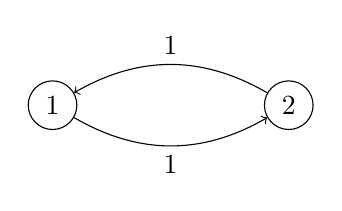
\begin{tikzpicture}
		\tikzstyle{line node} = [draw, fill=white, font=\footnotesize ]
	    \node[shape=circle,draw=black] (1) at (0,0) {1};
	    \node[shape=circle,draw=black] (2) at (3,0) {2};
	    \path [->](1) edge[bend right] node[midway,below] {$1$} (2);
	    \path [->](2) edge[bend right] node[midway,above] {$1$} (1);
	\end{tikzpicture}
\end{equation*}
Starting from $X_0=1$, it will be in state 1 at all even times and in state 2 at odd times — this chain is \emph{periodic}.
As a result, $p(X_t = i)$ alternates between 0 and 1 and does not converge over time.
But even though it has no limiting distribution, it does have a stationary distribution $\vecpi^\star = (\nicefrac{1}{2}, \nicefrac{1}{2})$, as is easily verified.




Here more more common thing that can go ‘wrong’: sinks can lead to multiple stationary distributions. 
Consider two connected copies of our weather model:
\begin{equation*}
	\begin{tikzpicture}
		\tikzstyle{line node} = [draw, fill=white, font=\footnotesize ]
	    \node[shape=circle,draw=black] (1) at (0,0) {1};
	    \node[shape=circle,draw=black] (2) at (2,0) {2};
	    \node[shape=circle,draw=black] (3) at (4,0) {3};
	    \node[shape=circle,draw=black] (4) at (6,0) {4};
	    \node[shape=circle,draw=black] (5) at (8,0) {5};
	
	    \path [->](1) edge[bend right] node[midway,below] {$\nicefrac{1}{2}$} (2);
	    \path [->](2) edge[bend right] node[midway,above] {$1$} (1);
	    \path [->](1) edge[out=135,in=225,looseness=8] node[midway,left] {$\nicefrac{1}{2}$} (1);
	    \path [->](3) edge node[midway,above] {$\nicefrac{1}{4}$} (2);
	    \path [->](3) edge node[midway,above] {$\nicefrac{3}{4}$} (4);
	    \path [->](4) edge[bend right] node[midway,below] {$\nicefrac{1}{2}$} (5);
	    \path [->](5) edge[bend right] node[midway,above] {$\nicefrac{1}{2}$} (4);
	    \path [->](5) edge[out=45,in=315,looseness=8] node[midway,right] {$1$} (5); 
	\end{tikzpicture}
\end{equation*}
If the chain at some point reaches node $2$ it will keep jumping between 1 and 2 afterwards. $\{1,2\}$ thus acts like a ‘sink’ from which there is no escape.
The set $\{4,5\}$ is another such sink.
Both sinks having their ‘own’ stationary distributions and
depending on the initial condition, the chain converges to one of them — or a mixture. 
Concretely, write $\delta_i$ for degenerate and deterministic distribution with all mass on state $i$.
If we start with the initial distribution $\vecpi_0 = \delta_1$, the chain converges to the stationary distribution $(\nicefrac{2}{3}, \nicefrac{1}{3}, 0, 0, 0)$.
But if we start on the other side with $\vecpi_0 = \delta_5$, then it converges to $(0,0,0,\nicefrac{1}{3}, \nicefrac{2}{3})$.
Finally, starting in the middle with $\vecpi_0 = \delta_3$ results in a mixture of both: $(\nicefrac{2}{12}, \nicefrac{1}{12}, 0, \nicefrac{3}{12}, \nicefrac{6}{12})$.
All of these are stationary distributions. 
(And so are all the convex combinations of $(\nicefrac{2}{3}, \nicefrac{1}{3}, 0, 0, 0)$ and $(0,0,0,\nicefrac{1}{3}, \nicefrac{2}{3})$.)




In this case, there is no unique stationary distribution because the graph has several sinks from which one cannot reach the other parts of the graph.
If \emph{every} state is reachable from every other state with positive probability in a finite number of steps, then it is called \emph{irreducible}.
Such a Markov chain has no sinks and every state will almost surely be visited again and again.\footnote{%
	%>>>
		This is generally not true for infinite state spaces, but introduced as an additional condition (\emph{recurrence})
	%<<<
	}
It (almost) never stops visiting the \emph{entire} state space.
	



%——————————————————————————————————————————————————————————
\paragraph{ergodicity}

Markov chains that are both irreducible and aperiodic are said to be \emph{ergodic}.
Together, the two properties are sufficient to ensure convergence of a Markov chain to a unique stationary distribution, just as in our weather model:
\begin{theorem}[1.8.3 in \cite{Norris1997}]
	\label{thm:convergence}
	Let $(x_0, x_1, \dots)$ be an ergodic Markov chain with initial distribution $\vecpi$, transition matrix $\mathbf{T}$ and stationary distribution $\vecpi^\star$. Then
	\begin{equation}
		p(x_n = i) \longrightarrow \pi_j^\star \quad \text{as} \quad n \longrightarrow \infty
	\end{equation}
	for all $i\in S$.
\end{theorem}




As we have seen, an ergodic Markov chain over time traverses the entire state space in an aperiodic fashion.
One might wonder if any regularity underlies the states it visits. 
Is it more likely to visit high-probability states under the stationary distribution, for example?
Indeed, it is.
The relative frequencies of visited states in fact converge to the stationary distribution. 
The important point is that this connects a distribution \emph{over time} — the visited states — with a distribution \emph{over the state space} — the stationary distribution.
\emph{Ergodic theory} studies this relation between time- and space-averages and I want to state one result here.
To do so we define these averages, for any bounded function $f: S \to \mathbb{R}$, as
\begin{equation}
	f_{\text{time}}	:= \frac{1}{n}\sum_{k=0}^{n-1} f(X_k)
		\quad\text{and}\quad
	f_{\text{space}} := \sum_{i\in S} \vecpi^\star_i f(i)
\end{equation}
The result is as follows.
\begin{theorem}[Ergodic Theorem; 1.10.2 in \cite{Norris1997}]
	Let $(x_n)_{n\ge 0}$ be as in theorem \ref{thm:convergence} and let $f: S \to \mathbb{R}$ be any bounded function. Then the time-average of $f$ almost surely converges to the space-average of $f$:
	\begin{equation}
		p\bigl(f_{\text{time}} \longrightarrow f_{\text{space}} \quad \text{as}\quad n \longrightarrow \infty \bigr) = 1.
	\end{equation}
\end{theorem}




I omit the proof, but want to draw a practical conclusion.
As seen, one can find the stationary distribution as an eigenvector of (an estimate of) the transition matrix, but the previous theorem shows a more intuitive option: measuring relative frequencies.
If $V_i(t)$ is the number of visits to state $i$ before time $t$, then $f_i(t) = V_i(t) / t$ is the relative frequency.
For an ergodic Markov chain, this converges to the stationary distribution,
$f_i(t) \to \pi_i$ as $t\to\infty$, with probability 1.
This is (a consequence of) the Ergodic theorem \parencite[][1.10.2]{Norris1997} when $f_i$ is the indicator function.
As the reader might notice, this fact has been used extensively.



%——————————————————————————————————————————————————————————
\showbibliography



\end{document}